\chapter{Device Design}
\label{chap:design}


In this chapter, the resulting cloning device, its hardware and software will be designed. The selection of components is based on the Chapter~\ref{chap:analysis}.

\section{Hardware}

After a thorough selection of hardware components, the best combination of the Proxmark 3 Easy reader with a Raspberry Pi 4 B microcomputer was found. These two devices will be connected by a USB-to-micro USB cable, where the male ends can be connected with the shortest possible connection cable to save space in the final device. This cable will provide all communication between the microcomputer and the reader, and will also power the Proxmark 3 Easy via this cable. On the Raspberry Pi itself, a Waveshare 3.5" LCD touchscreen will be connected via pins, which is the size of a microcomputer. The image will be transmitted via the pins and the screen will be powered via this route. An illustration of the component wiring can be seen in the Figure~\ref{fig:devicescheme}. 


\begin{figure}[ht]
  \centering
  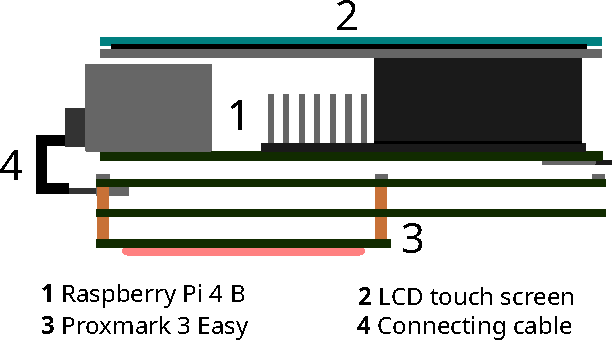
\includegraphics[width=6cm]{text/device_scheme.pdf}
  \caption[Illustration of component wiring.]{~Illustration of component wiring.}
  \label{fig:devicescheme}
\end{figure}

To ensure greater battery life and the renewability of the power source, it is best to power the device using a power bank, which will be connected externally to the device using a classic USB-C cable. It is recommended that the power bank supplies the device with 5V/3A~\cite{raspberrydoc}.

This design makes the device compact and easy to use. On the top touch screen, the user controls the device and attaches cloned tags from the bottom of the device. It should be noted that the Proxmark 3 Easy has the LF and HF antenna in different locations, the user must then attach the tag to the specific antenna as needed.

The Proxmark has a button on its longer side that is used to control some of its functions. It is important because card emulation is terminated with this button. It is therefore necessary to make this button accessible to the user.


\section{Software}

This section will justify the selection of the software parts of the project.

\subsection{Operating System}

With the selection of the Raspberry Pi microcomputer, it became clear that Linux would be used as the operating system of the device. It is possible to choose a specific Linux distribution, but for this purpose the official Raspberry Pi OS, which can be obtained for free from the Raspberry~Pi~\cite{raspberrypios} website, will suffice.

The instructions for installing the LCD touch screen drivers recommend the Linux version of bullseye, 32 bit. For the purposes of this device, this version of Linux is suitable.~\cite{waveshare35inch}

The operating system will run in the background of the device, the user will not be able to manipulate the operating system in any way --- and therefore, when Linux starts, the program created will automatically run and take up the entire screen. When the program is finished, the computer itself will shut down. A slight but tolerable drawback is the startup time.

Since the device will be controlled by touch screen, the operating system will have to be adapted to this, and therefore at least make the mouse cursor invisible.

\subsection{Communication With Proxmark}
\label{subsec:communication}

Proxmark 3 Easy is controlled via the commandline client, see Figure~\ref{fig:pm3}. Single commands are sent to the reader to perform operations, such as reading or writing tags. It is also possible to start the client to perform only one specific operation. An output is sent back from Proxmark, which contains various information, such as the success of the operations, or an enumeration of the tag contents. The created program will therefore communicate with Proxmark by starting a process where it sends a specific operation to Proxmark for execution, then parsing the output and passing the necessary feedback to the user. It will also need to ensure that the program checks the availability of Proxmark to avoid errors.

\begin{figure}[ht]
  \centering
  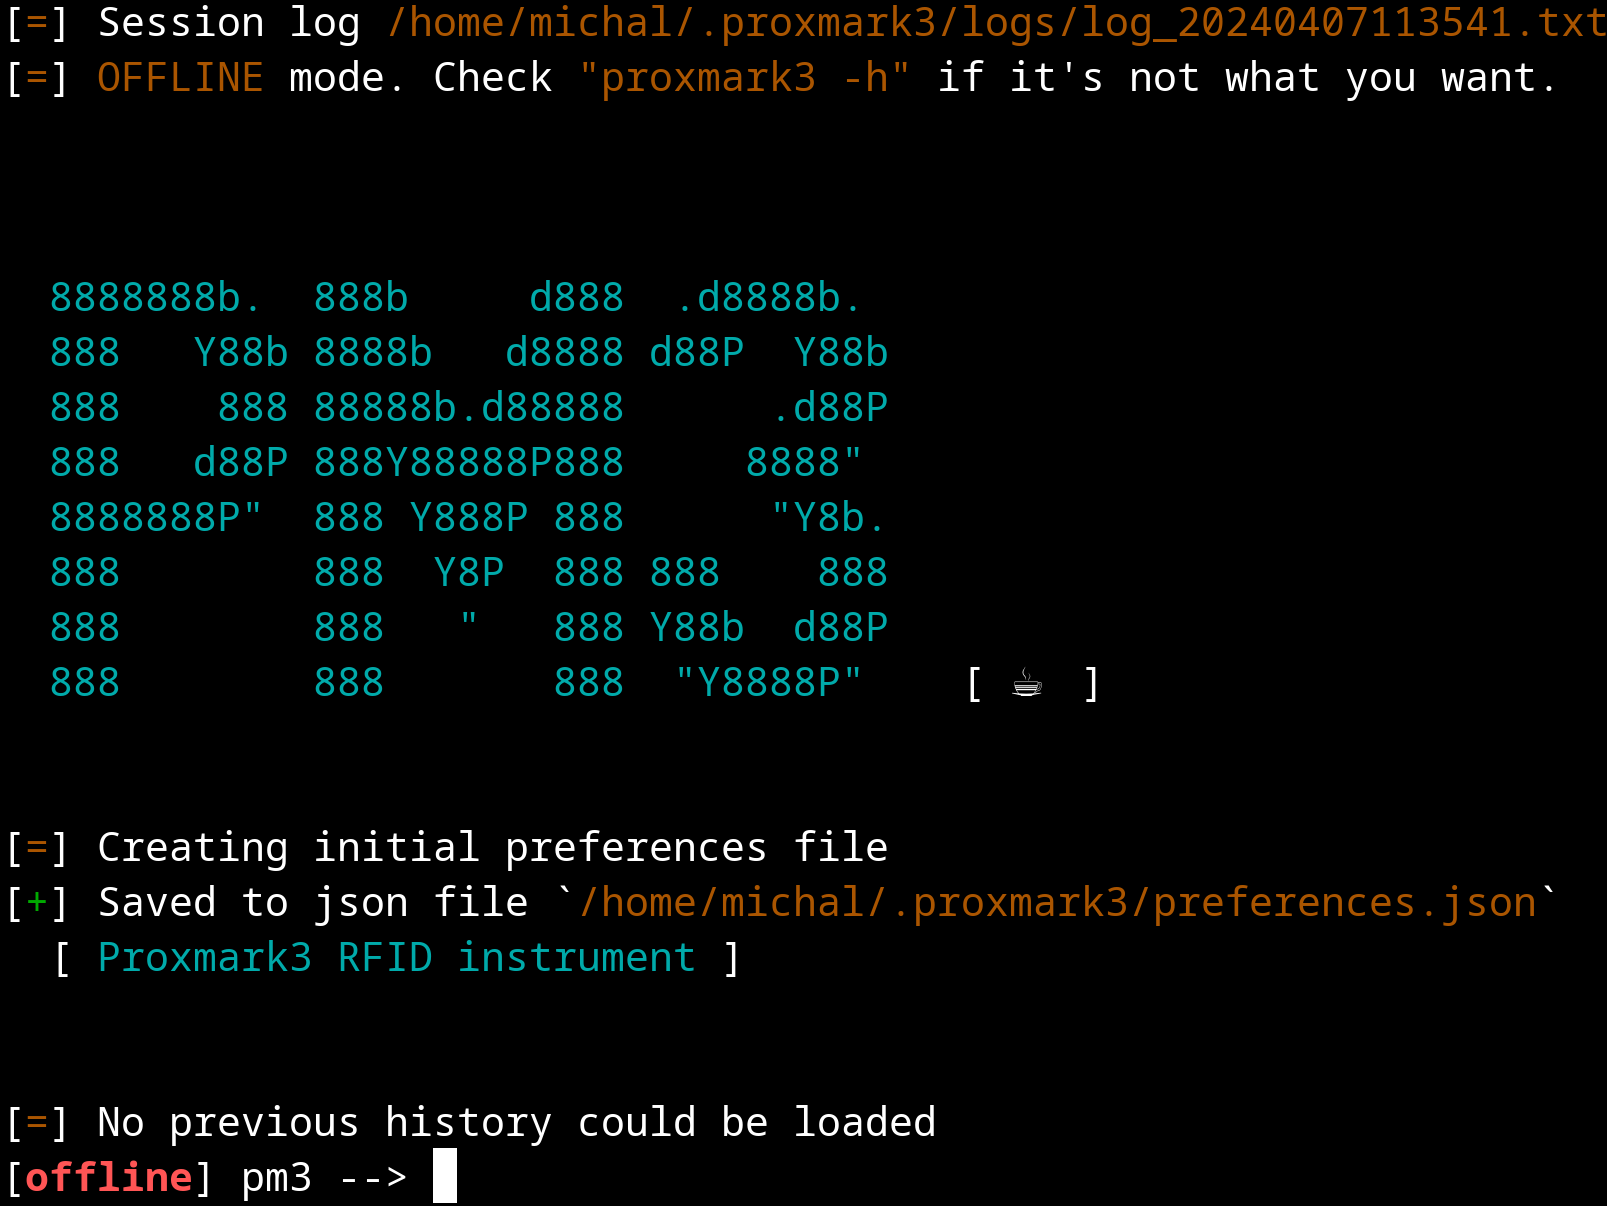
\includegraphics[width=10cm]{text/pm3.png}
  \caption{~Preview of Proxmark commandline client.}
  \label{fig:pm3}
\end{figure}

Some Proxmark operations, such as emulation of some tag types, cannot be terminated by user input in the client, but by pressing a physical button on the Proxmark itself. For this reason, the button will need to be accessible.


\subsection{Programming Language}

The Subsection~\ref{subsec:communication} shows that the program with the graphical environment itself will not actually do any complex calculations, it will only send commands to Proxmark and parse the output. For this reason, the Python programming language is an excellent choice. Man can choose from quite a few graphical libraries to create a graphical interface, and parsing the output is very straightforward.

\subsubsection{Python Graphical User Interface Library}

There are no big demands on the GUI library, from many suitable ones such as PyQt5~\cite{pythonpyqt5}, Kivy~\cite{pythonkivy}, or TKinter~\cite{pythontkinter} the PyQt5 library was chosen, which coincidentally is already part of the Rasperry Pi Os Bullseye 32 bit operating system. This library provides everything needed to create a GUI program.


\subsection{Program}

The program itself must therefore give the user the ability to easily control Proxmark. It must allow the user the following functions:

\begin{itemize}
    \item display basic information about the attached tag,
    \item dumping and storing data of different tag types,
    \item cloning saved dumps into new tags,
    \item manually edit the UIDs of different tag types,
    \item emulate the content of different tag types and
    \item emulate UIDs of different tag types.
\end{itemize}

When it comes to displaying various information about the attached tag, the Proxmark output itself is already clear and needs almost no editing.

Storing tag dump data will force the existence of a repository in Proxmark where the dumps will be stored. The program itself will then need to include an interface where the user can browse these files.

Manual editing of UIDs will require some sort of on-screen keyboard where the user can enter input. There is a solution of a pop-up keyboard, but a more elegant solution is to create a custom keyboard where only the keys that are needed will be present. The UID is simply read in hexadecimal format, so it will be sufficient if the keyboard contains only the characters 0--9 and A--F.

\subsubsection{Architecture}

The PyQt5 library offers a relatively simple way to manage individual screens. The QStackedWidget class will allow you to hold individual widgets\footnote{Widget is the class representing the screen for us at the moment}. Inside the widget, the screen layout can be arranged in a simple way by aligning or applying individual styles. Each screen, i.e. widget, will hold its sub-screens (submenus). This hierarchy allows for easy navigation through the code.

Next, you will need to have a class, let's call it CommandExecutor, which will take care of executing individual operations on the Proxmark.

A class called CommandBuilder will prepare individual commands for the CommandExecutor class to execute, depending on the user's input.

And of course, you will also need to have a class that will process the output received from the Proxmark, and forward the signals back to the user.

For working with files it will be useful to create a class with methods that will take care of this work. 

For easier debugging, it will be smart from the beginning to implement a logging system that will store all logs in a file and that can be looked at and evaluated later.

The process of executing a command --- how the classes will pass information to each other can be seen in Figure~\ref{fig:architecture}.

\begin{figure}[ht]
  \centering
  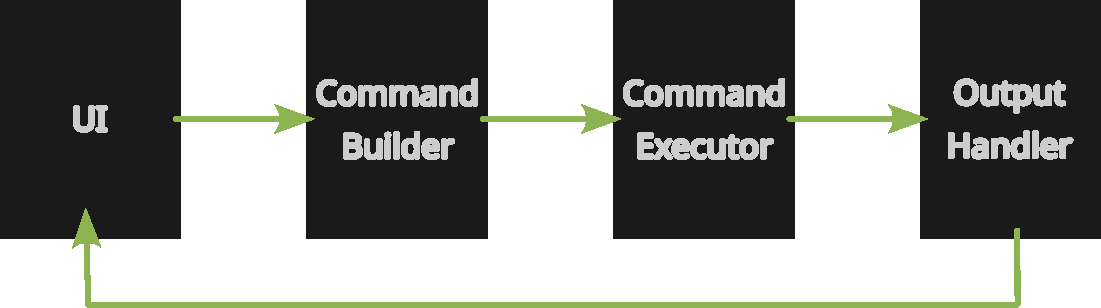
\includegraphics[width=\textwidth]{text/architecture.pdf}
  \caption{~Information flow between classes.}
  \label{fig:architecture}
\end{figure}


\subsubsection{GUI Design}

First of all, it is important to design how the user interface of the program will look like. Since it will run on a small display with a resolution of only 480 × 320, the GUI must be well laid out and easy to use.

To keep it simple, the best solution will be to create some menus and submenus that the user will navigate back and forth through. This will ensure simplicity of operation on the touchscreen and allow for a relatively small number of buttons in a single menu. This will ensure that everything will always fit on the small screen and there will be no problem with lack of space. In some situations, however, there may be a problem that more content needs to be displayed than can fit on one screen, for example when displaying a list of saved tags. Such a situation can be solved by inserting a scrolling area, where it will be possible to scroll in the user interface.

To get an idea of how such an interface would look like, we can refer to Figure~\ref{fig:wireframe1}, Figure~\ref{fig:wireframe2} and Figure~\ref{fig:wireframe3} containing black and white wireframes.


\begin{figure}[h]
    \centering
    \begin{minipage}[b]{0.315\textwidth}
        \centering
        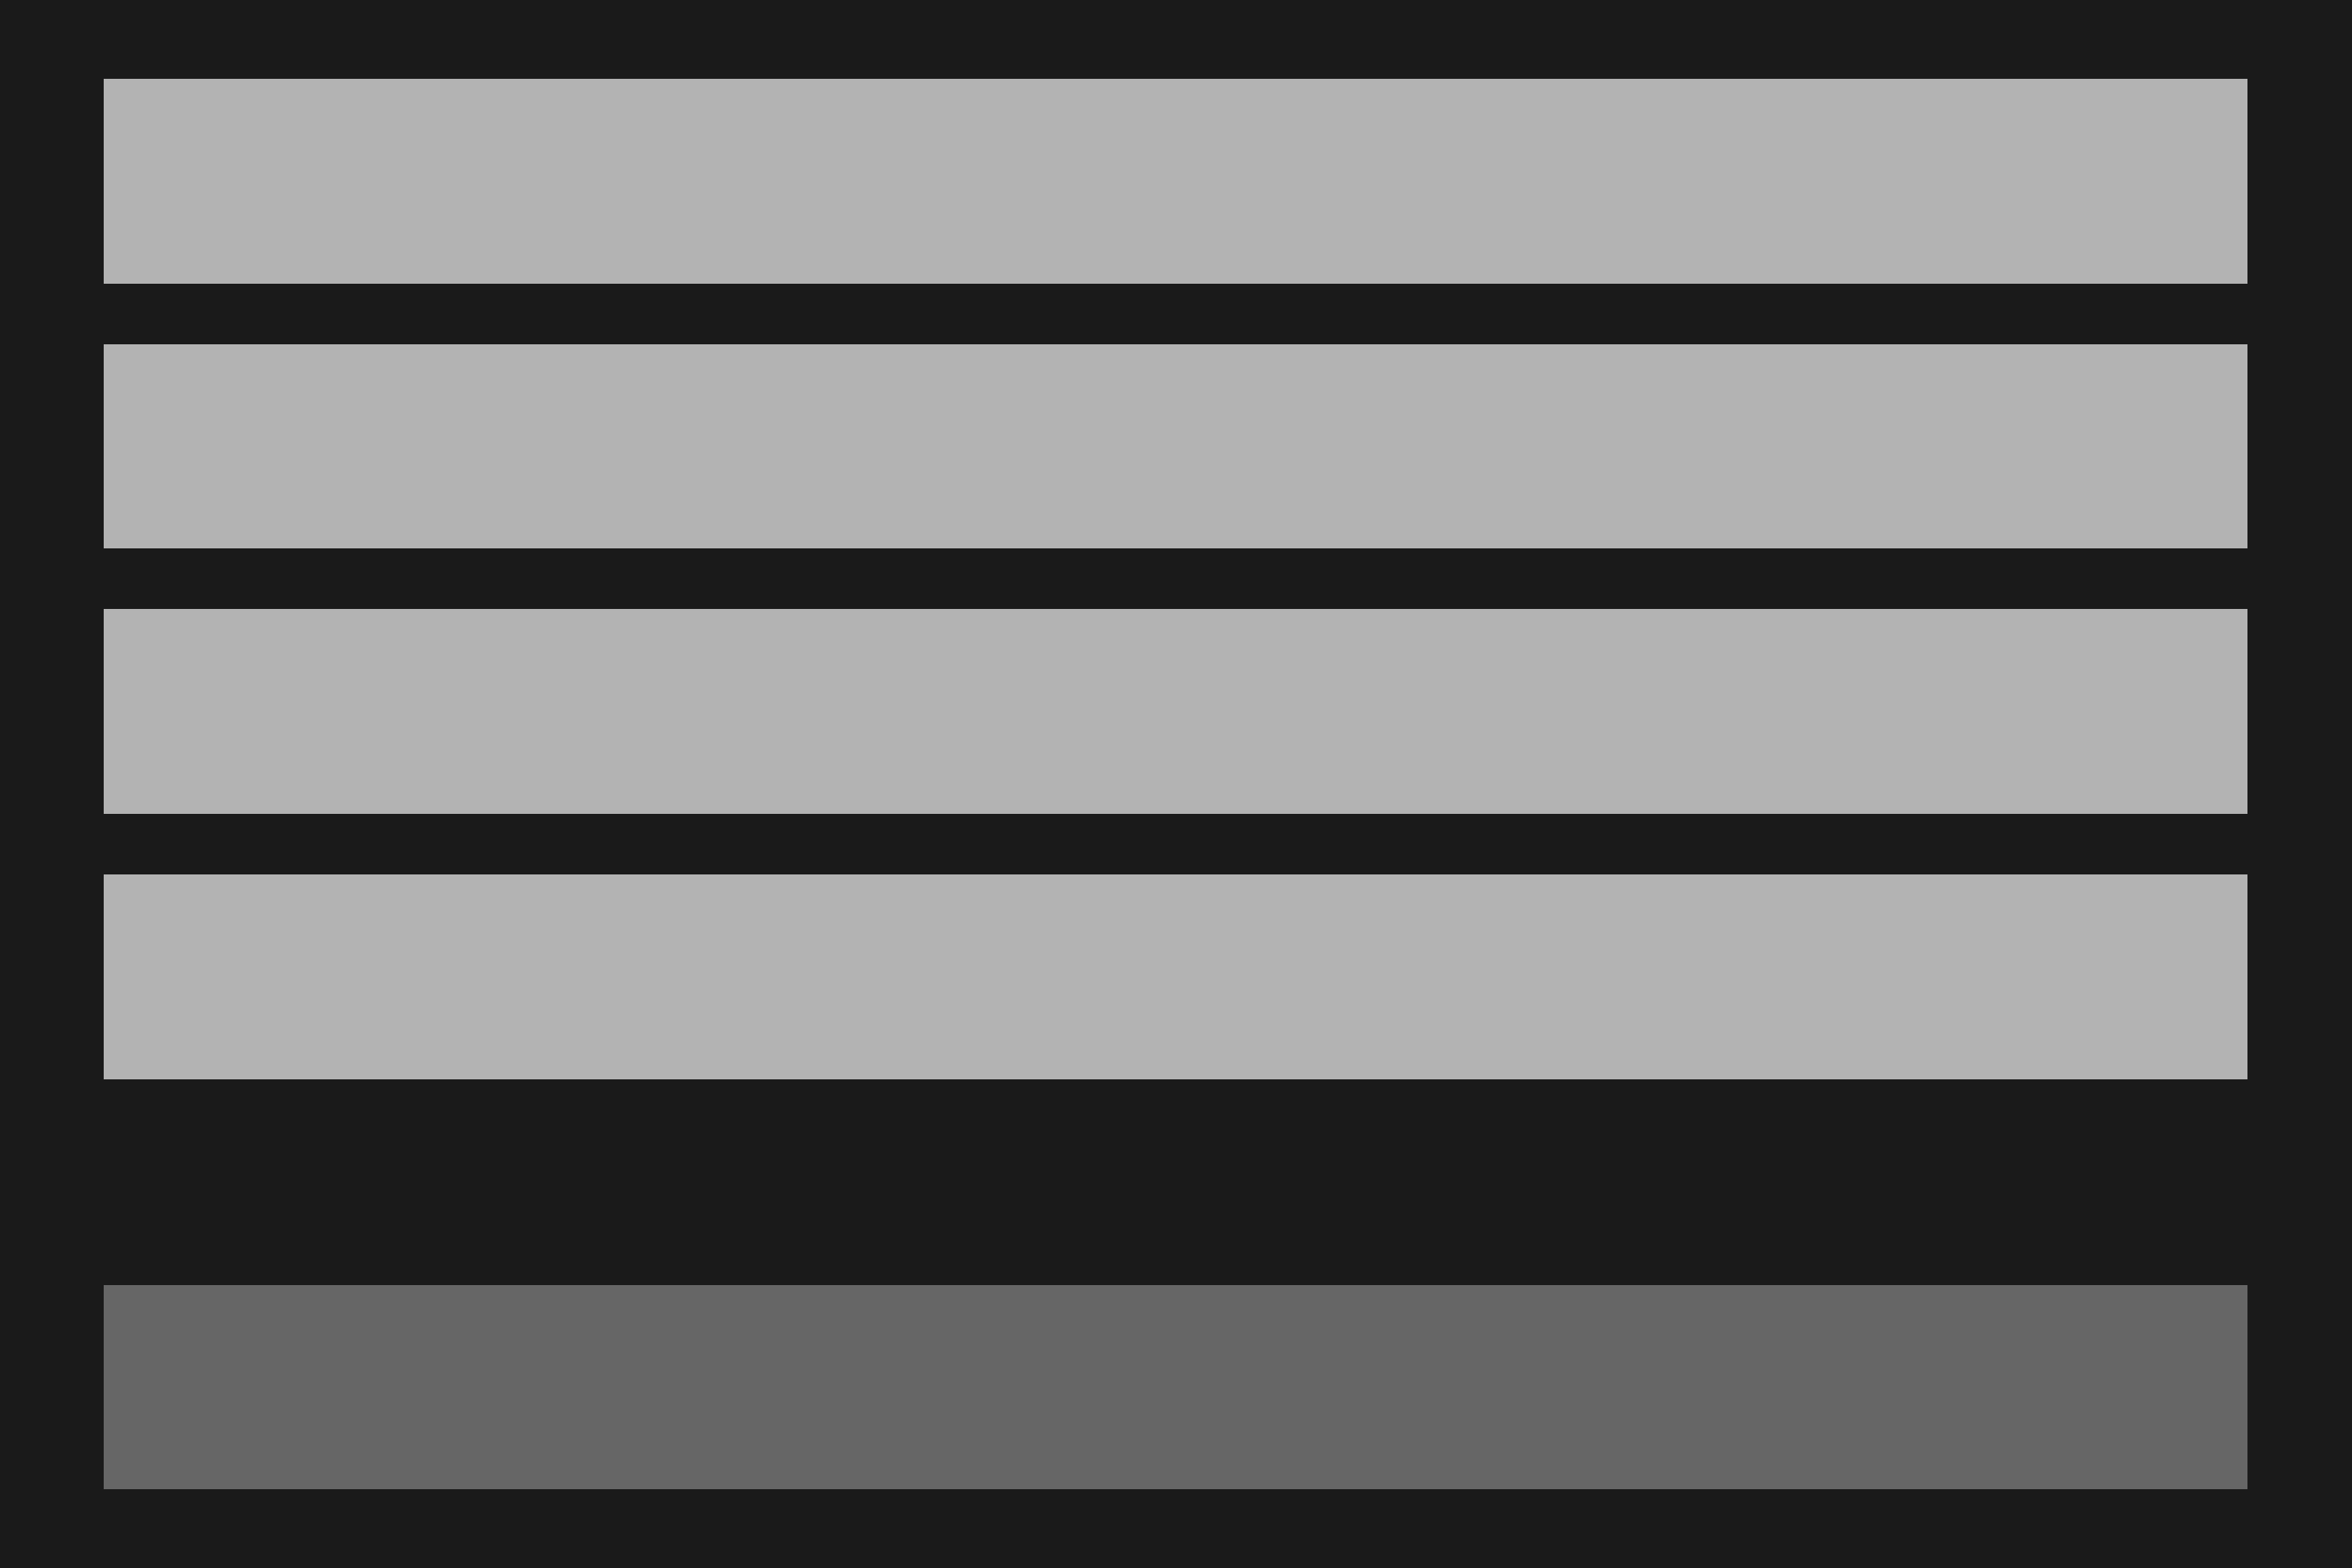
\includegraphics[width=\textwidth]{text/wireframe1.pdf}
        \caption{~Wireframe 1.}
        \label{fig:wireframe1}
    \end{minipage}
    \hfill
    \begin{minipage}[b]{0.315\textwidth}
        \centering
        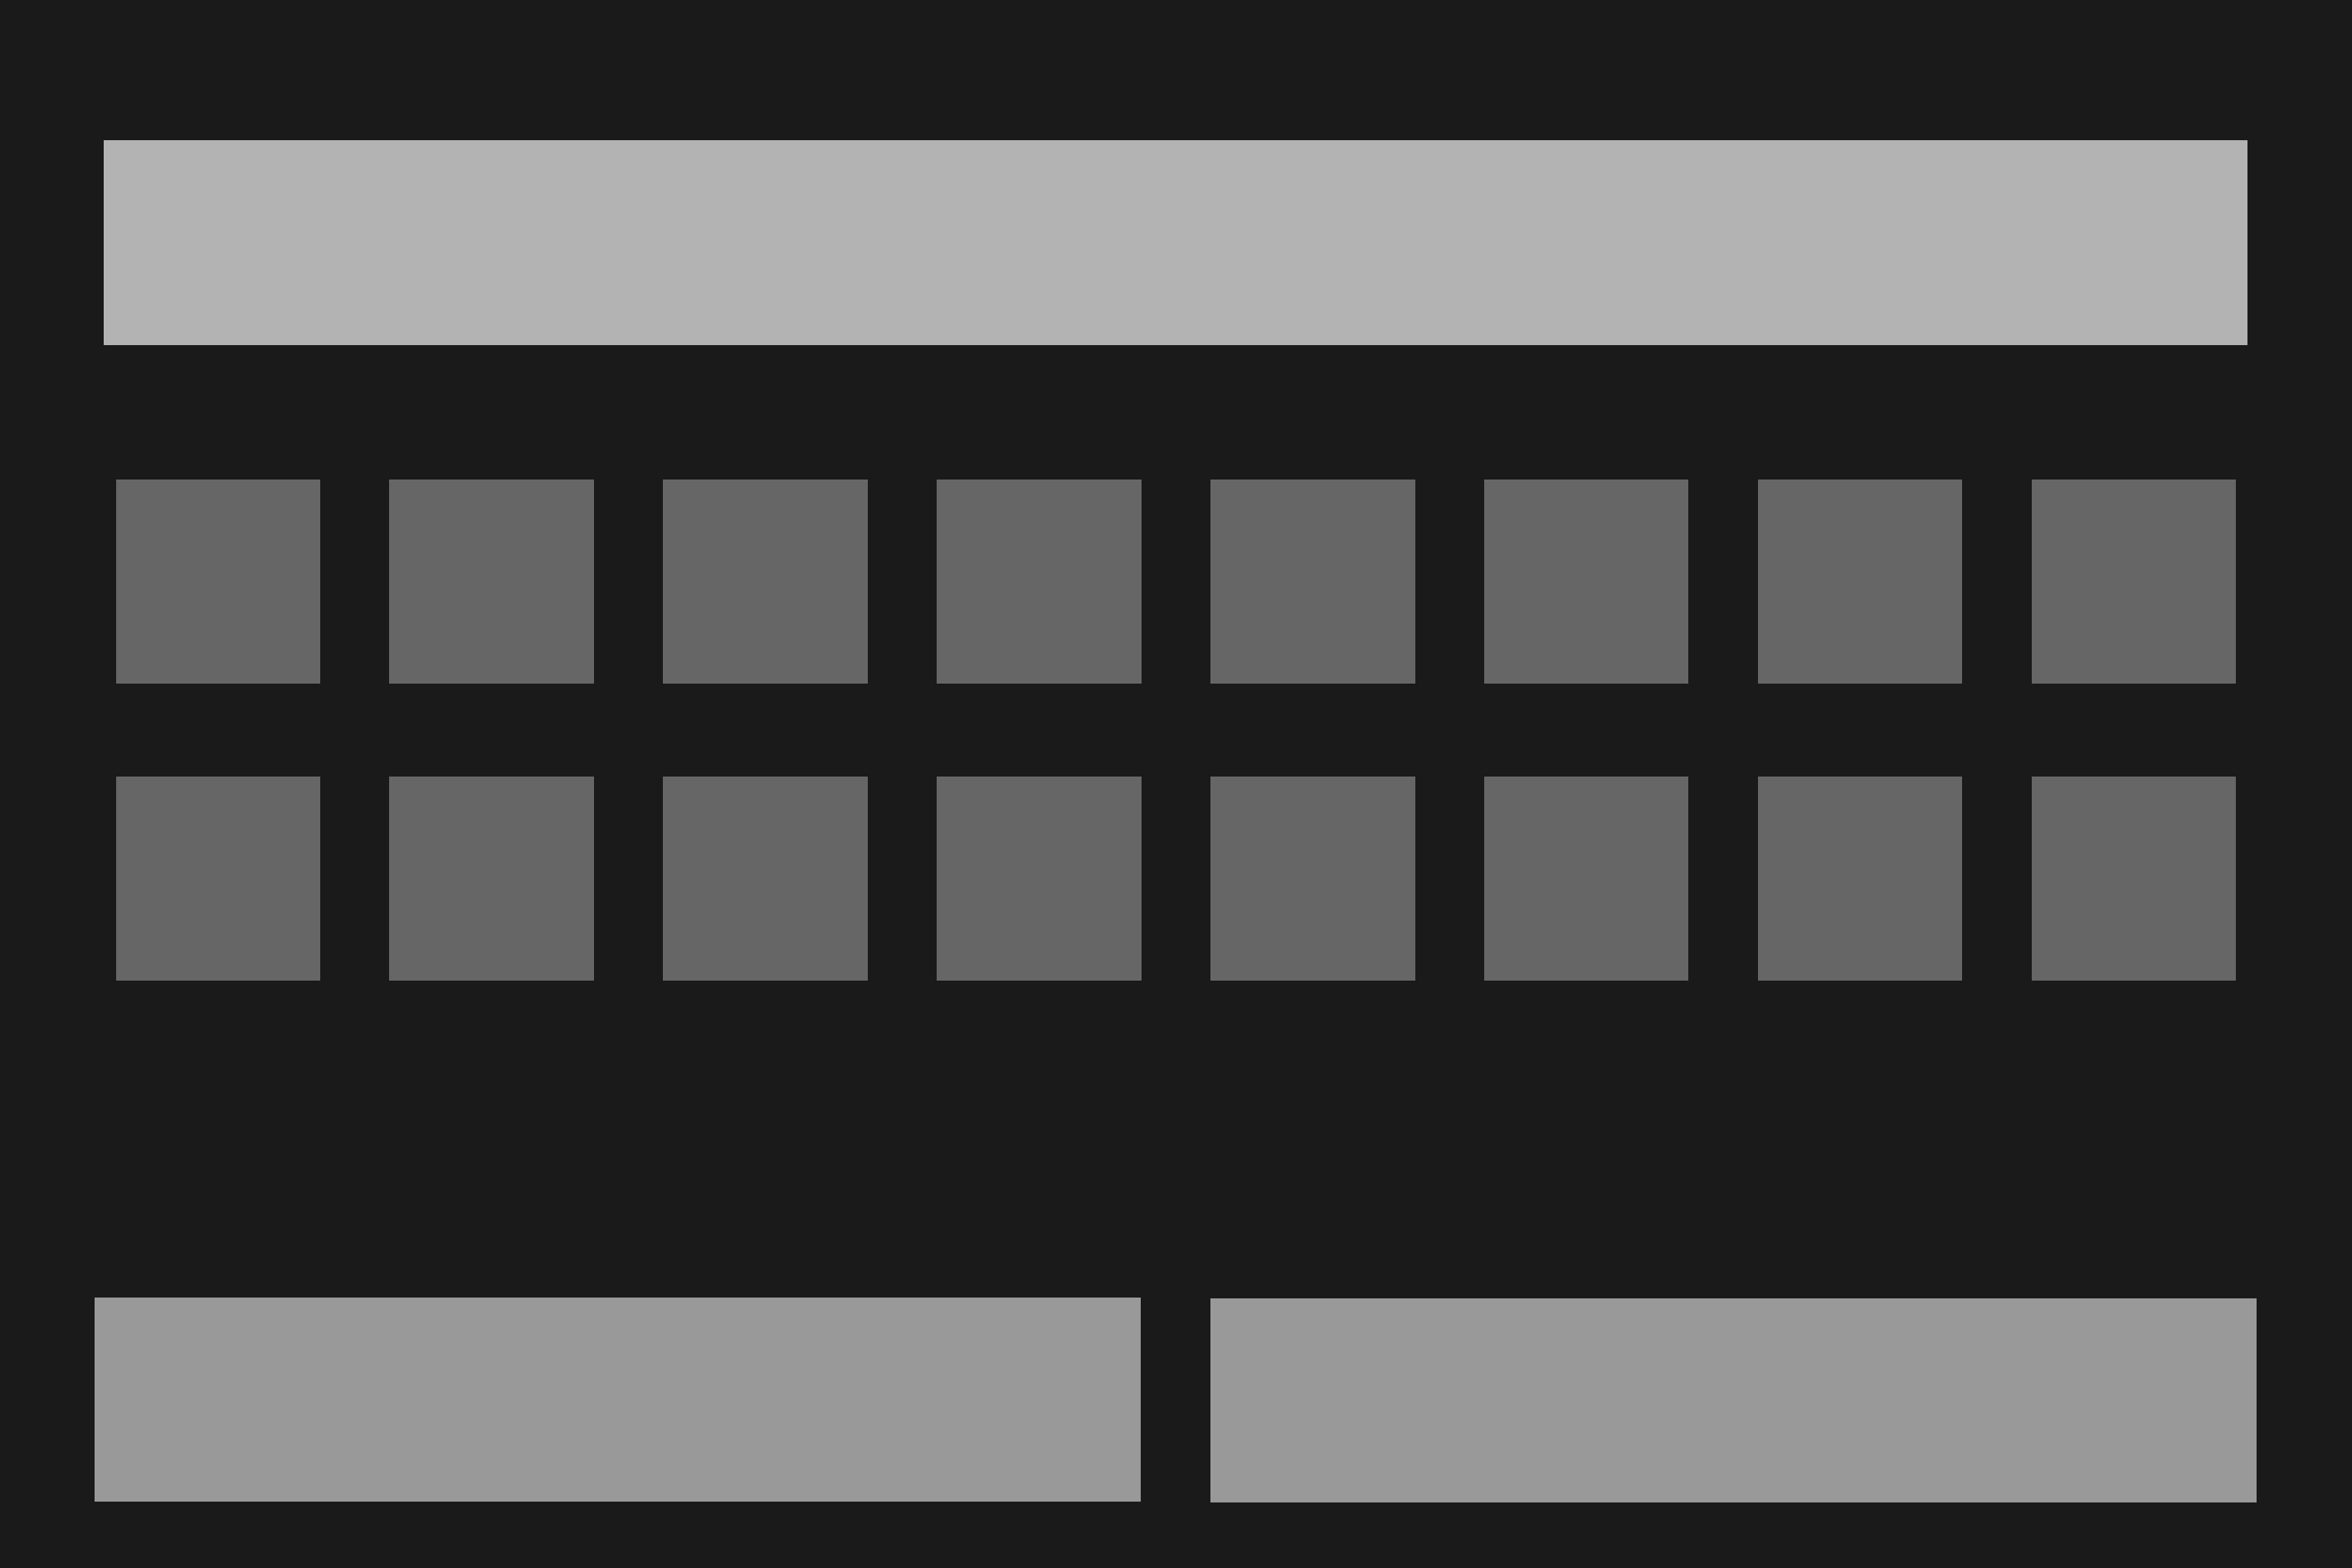
\includegraphics[width=\textwidth]{text/wireframe2.pdf}
        \caption{~Wireframe 2.}
        \label{fig:wireframe2}
    \end{minipage}
    \hfill
    \begin{minipage}[b]{0.315\textwidth}
        \centering
        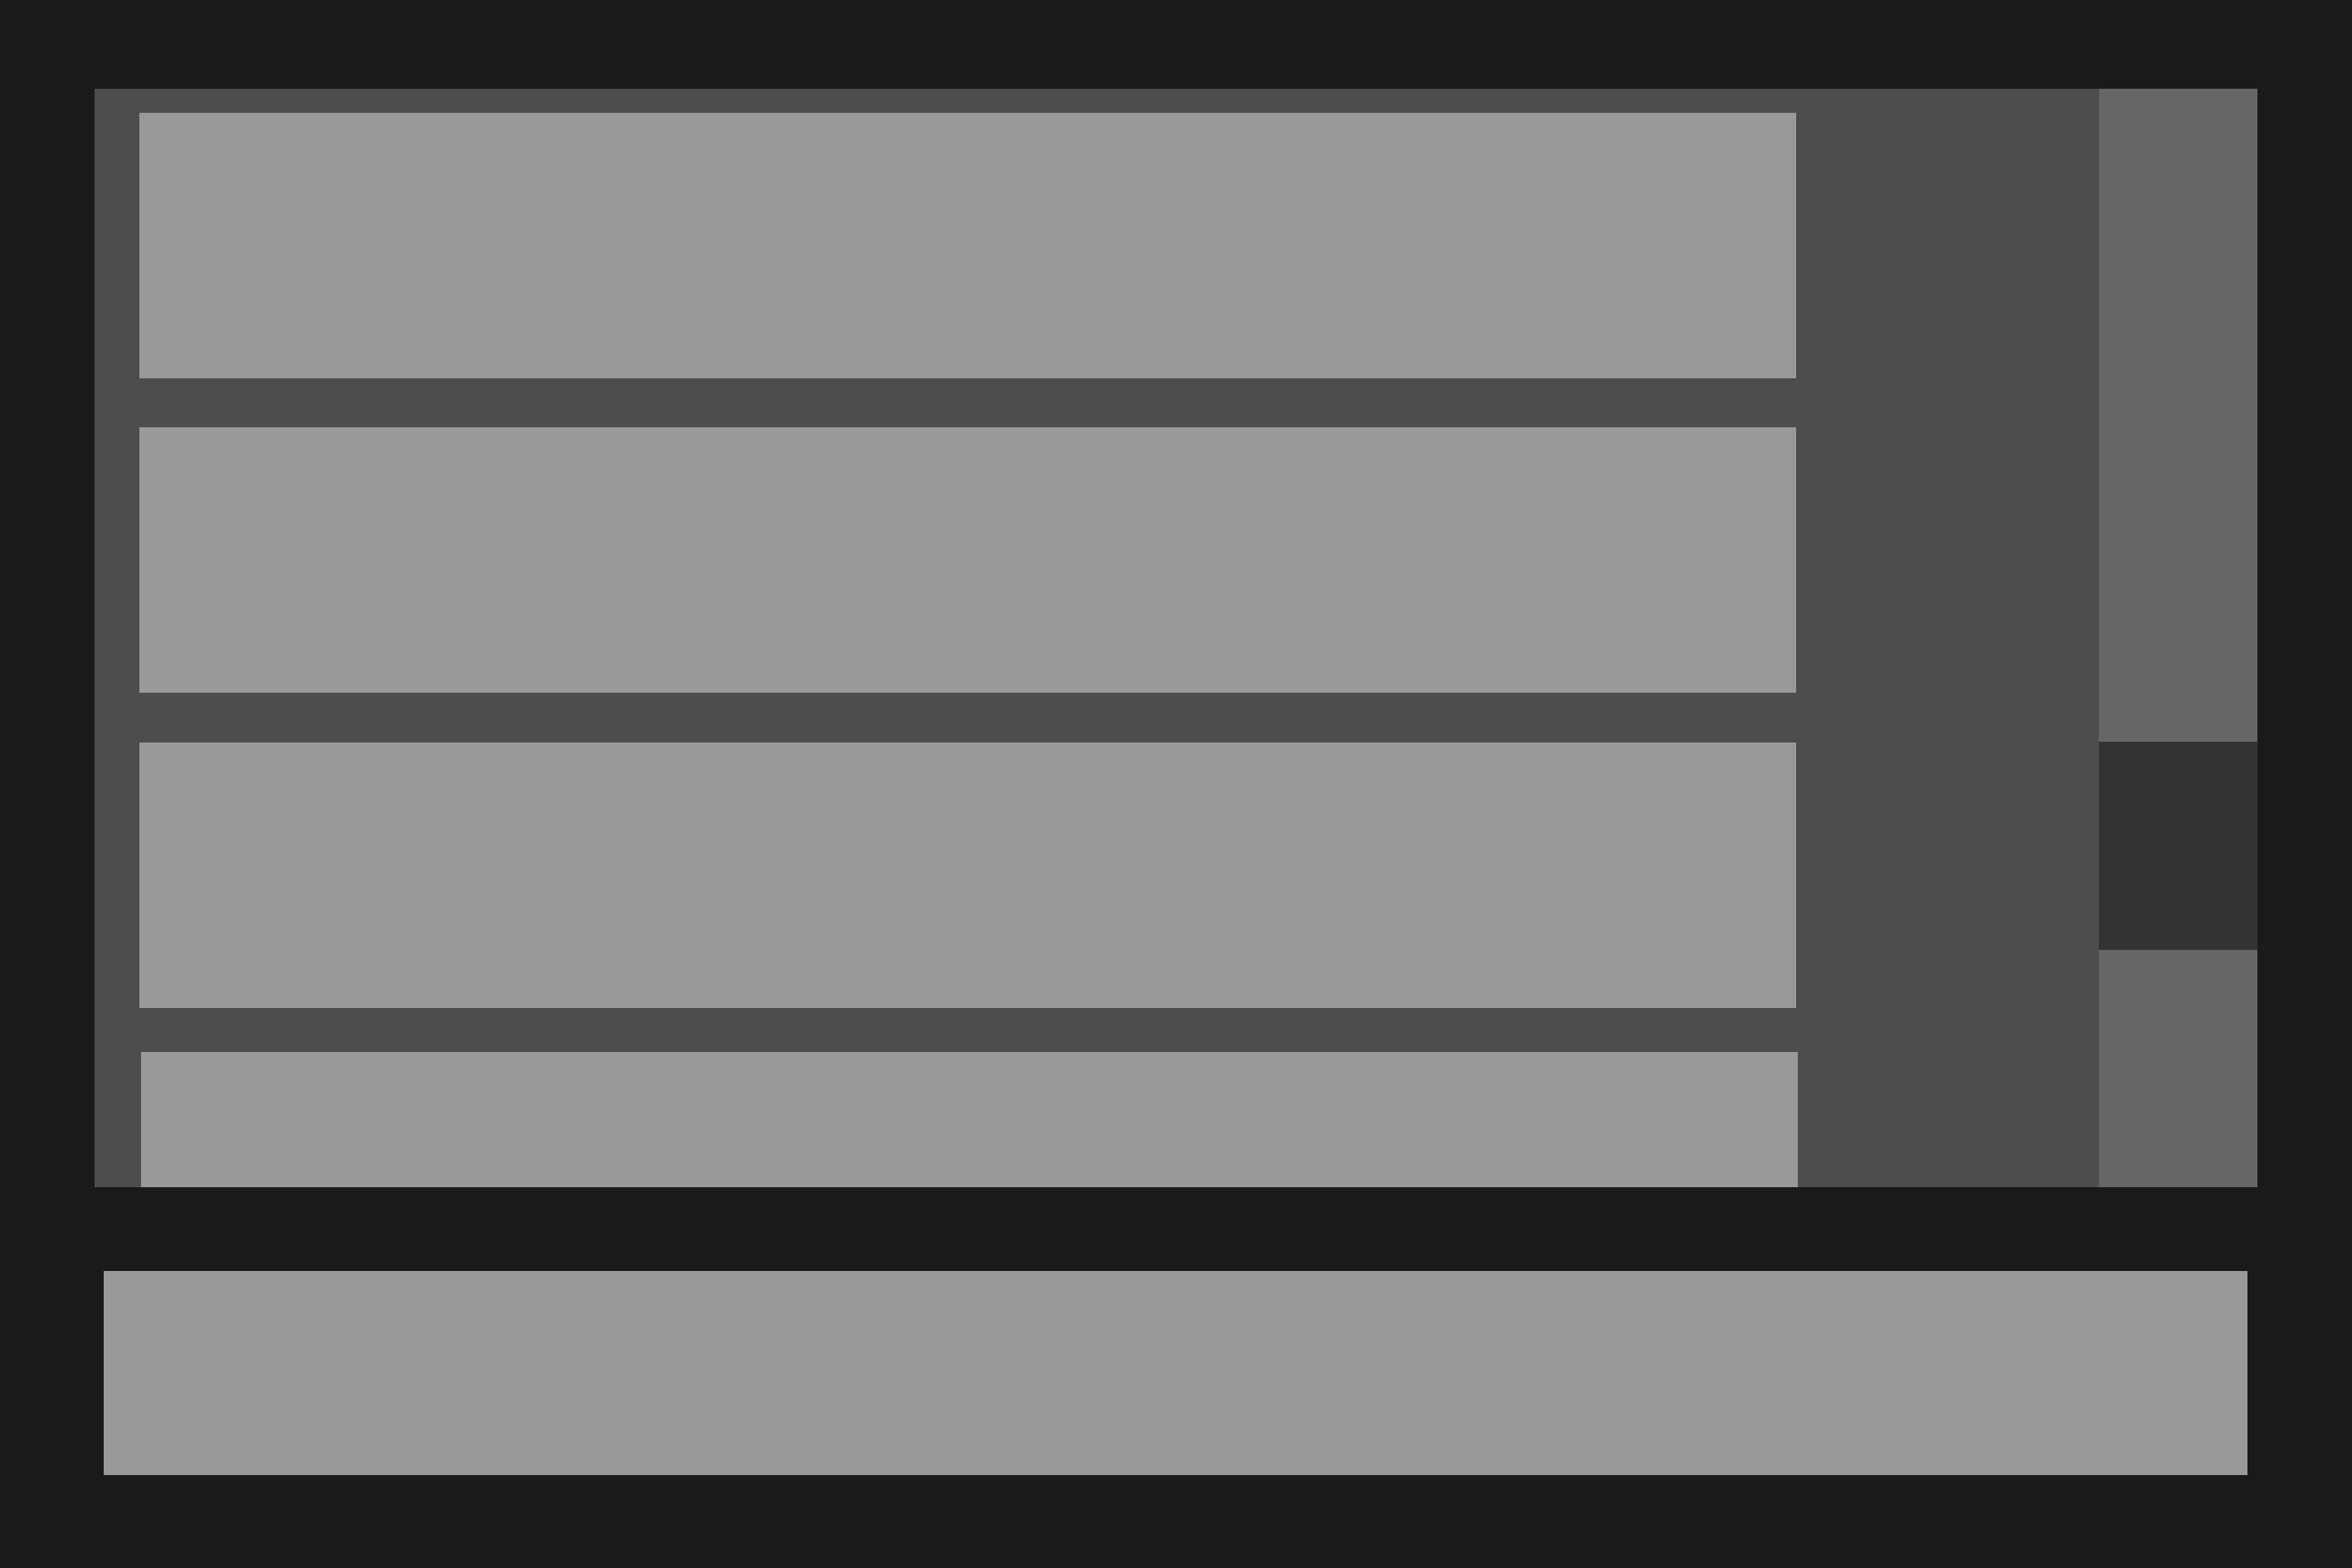
\includegraphics[width=\textwidth]{text/wireframe3.pdf}
        \caption{~Wireframe 3.}
        \label{fig:wireframe3}
    \end{minipage}
\end{figure}

